% ============================================================================
% Paper IV: Planner Engine — Market-Driven Task Orchestration in Elixir/OTP
% Part IV of V: "The AI Operating System" Series
% GrokRxiv:2026.03.planner-engine-ai-os [cs.AI] 10 Mar 2026
% ============================================================================
\documentclass[12pt,a4paper]{article}

% --- Core packages ---
\usepackage[utf8]{inputenc}
\usepackage[T1]{fontenc}
\usepackage{lmodern}
\usepackage[margin=1in]{geometry}
\usepackage{amsmath,amssymb,amsthm,mathtools}
\usepackage{tikz}
\usetikzlibrary{arrows.meta,positioning,decorations.pathmorphing,calc,shapes.geometric}
\usepackage{listings}
\usepackage[ruled,vlined,linesnumbered]{algorithm2e}
\usepackage{hyperref}
\usepackage{cleveref}
\usepackage{enumitem}
\usepackage{booktabs}
\usepackage{multirow}
\usepackage{xcolor}
\usepackage{float}
\usepackage{caption}
\usepackage{subcaption}
\usepackage{graphicx}
\usepackage{microtype}
\usepackage{authblk}
\usepackage{abstract}
\usepackage{fancyhdr}
\usepackage{everypage}

% --- GrokRxiv sidebar ---
\definecolor{grokgray}{RGB}{110,110,110}
\AddEverypageHook{%
  \ifnum\value{page}=1
    \begin{tikzpicture}[remember picture, overlay]
      \node[
        rotate=90,
        anchor=south,
        font=\Large\sffamily\bfseries\color{grokgray},
        inner sep=0pt
      ] at ([xshift=38pt, yshift=0.52\paperheight]current page.south west)
      {GrokRxiv:2026.03.planner-engine-ai-os\quad
       [\,cs.AI\,]\quad
       10 Mar 2026};
    \end{tikzpicture}
  \fi
}

% --- Colors ---
\definecolor{elixirpurple}{RGB}{75,0,130}
\definecolor{elixirgreen}{RGB}{0,128,0}
\definecolor{elixirblue}{RGB}{0,70,140}
\definecolor{elixirred}{RGB}{180,0,0}
\definecolor{codebg}{RGB}{248,248,248}
\definecolor{codeframe}{RGB}{200,200,200}

% --- Listings config ---
\lstdefinelanguage{elixir}{
  morekeywords={defmodule,def,defp,do,end,use,require,import,alias,case,cond,if,else,unless,
    fn,when,with,for,receive,after,try,catch,rescue,raise,throw,quote,unquote,
    defstruct,defprotocol,defimpl,defmacro,defmacrop,defguard,defdelegate,
    true,false,nil,and,or,not,in,GenServer,Supervisor,Application},
  sensitive=true,
  morecomment=[l]{\#},
  morecomment=[s]{@doc\ \"\"\"}{\"\"\" },
  morestring=[b]",
  morestring=[b]',
  literate={|>}{{{\color{elixirpurple}|>}}}2
           {->}{{{\color{elixirpurple}->}}}2
           {=>}{{{\color{elixirpurple}=>}}}2
           {<-}{{{\color{elixirpurple}<-}}}2,
}

\lstset{
  language=elixir,
  basicstyle=\ttfamily\small,
  keywordstyle=\color{elixirpurple}\bfseries,
  commentstyle=\color{elixirgreen}\itshape,
  stringstyle=\color{elixirred},
  backgroundcolor=\color{codebg},
  frame=single,
  rulecolor=\color{codeframe},
  breaklines=true,
  breakatwhitespace=true,
  numbers=left,
  numberstyle=\tiny\color{gray},
  numbersep=8pt,
  tabsize=2,
  showstringspaces=false,
  captionpos=b,
  aboveskip=1em,
  belowskip=1em,
}

% --- Theorem environments ---
\theoremstyle{plain}
\newtheorem{theorem}{Theorem}[section]
\newtheorem{lemma}[theorem]{Lemma}
\newtheorem{proposition}[theorem]{Proposition}
\newtheorem{corollary}[theorem]{Corollary}
\theoremstyle{definition}
\newtheorem{definition}[theorem]{Definition}
\newtheorem{example}[theorem]{Example}
\newtheorem{remark}[theorem]{Remark}
\newtheorem{invariant}[theorem]{Invariant}

% --- Header ---
\pagestyle{fancy}
\fancyhf{}
\fancyhead[L]{\small Paper IV: Planner Engine}
\fancyhead[R]{\small The AI Operating System}
\fancyfoot[C]{\thepage}
\renewcommand{\headrulewidth}{0.4pt}

% ============================================================================
\begin{document}

\title{\textbf{The AI Operating System, Part IV:}\\[0.5em]
\Large Planner Engine --- Market-Driven Task Orchestration\\
in Elixir/OTP}

\author{Matthew Long\\
The YonedaAI Collaboration\\
YonedaAI Research Collective\\
Chicago, IL\\
\texttt{matthew@yonedaai.com} $\cdot$ \texttt{https://yonedaai.com}}

\date{March 10, 2026}

\maketitle
\thispagestyle{fancy}

% ============================================================================
% ABSTRACT
% ============================================================================
\begin{abstract}
\noindent
We present the design and implementation of a \emph{planner engine} for an AI operating system---the highest-level orchestration primitive, analogous to \texttt{systemd}/\texttt{init} in classical operating systems. Rather than scheduling deterministic processes, this planner coordinates a marketplace of self-interested AI agents through five collaborating Elixir/OTP subsystems: (1)~an \emph{order book} GenServer implementing demand/supply matching with composite scoring across reputation, capability, and price; (2)~an \emph{escrow} system backed by Mnesia transactions providing atomic hold/settle/refund operations with conservation guarantees; (3)~a \emph{task decomposer} that breaks complex jobs into directed acyclic graphs with topological sorting for parallel execution scheduling; (4)~a \emph{market clearing} module managing the full contract lifecycle from proposal acceptance through revenue distribution (70/15/15 operator/platform/LLM split); and (5)~a \emph{reputation engine} computing exponentially-weighted 6-dimensional quality scores with anti-gaming detection for score inflation, rapid cycling, and perfect-streak anomalies. The system is built entirely on OTP patterns---GenServer state machines, Supervisor fault tolerance, Mnesia transactional storage, and pipeline composition via the \texttt{|>} operator---and maps directly to a production AI agent marketplace where jobs follow the lifecycle \texttt{draft} $\to$ \texttt{open} $\to$ \texttt{in\_progress} $\to$ \texttt{review} $\to$ \texttt{completed}. We show how algebraic data types and pattern matching yield an implementation that is both formally precise and operationally robust.

\medskip
\noindent\textbf{Keywords:} AI planning, order book, escrow, market clearing, task decomposition, reputation systems, Elixir/OTP, GenServer, Mnesia, agent marketplace, pipeline composition
\end{abstract}

\vspace{1em}

% ============================================================================
% 1. INTRODUCTION
% ============================================================================
\section{Introduction}\label{sec:introduction}

Every operating system has a process that runs first and orchestrates everything else. In Unix, this is \texttt{init} (PID~1). In modern Linux, \texttt{systemd} manages service dependencies, socket activation, and lifecycle transitions. In Kubernetes, the scheduler assigns pods to nodes based on resource requests, affinity rules, and priority classes. These systems solve the same fundamental problem: given a set of work items and a set of executors, determine \emph{who does what, when, and how}.

An AI operating system faces this problem at a higher level of abstraction. The ``processes'' are not deterministic programs but stochastic agents with heterogeneous capabilities, varying reliability, and economic incentives. The ``scheduler'' must not only assign tasks but must negotiate prices, hold funds in escrow, verify quality, and update reputations. The planner engine of an AI OS is simultaneously:

\begin{enumerate}[label=(\roman*)]
    \item A \textbf{task decomposer} that breaks complex jobs into dependency graphs of subtasks;
    \item A \textbf{marketplace} where agents bid on work and clients select providers;
    \item A \textbf{financial system} managing credits, escrow, and revenue distribution;
    \item A \textbf{reputation engine} that scores quality and detects gaming.
\end{enumerate}

This paper presents a complete design and implementation of such a planner engine in Elixir/OTP, emphasizing the use of functional programming patterns---algebraic data types, pattern matching, GenServer state machines, Mnesia transactions, supervision trees, and pipeline composition---to achieve an architecture that is both formally clean and production-ready.

\paragraph{Why Elixir/OTP.} The BEAM virtual machine provides three properties that are uniquely suited to marketplace orchestration. First, \emph{lightweight processes} allow each component (order book, escrow, reputation, market) to run as an independent GenServer with isolated state, communicating through message passing. Second, \emph{supervision trees} with the let-it-crash philosophy mean that a failure in the reputation engine does not bring down the escrow system---the supervisor simply restarts the failed child. Third, \emph{Mnesia} provides distributed, transactional storage that runs in the same BEAM node, eliminating the network hop to an external database for latency-critical financial operations.

\paragraph{Categorical context.} The structures in this paper have natural interpretations in category theory: the order book is a profunctor, escrow operations form a monad, market clearing is a colimit, and task decomposition is a functor. We note these connections where they illuminate the design, but the primary language of this paper is that of functional programming and system design. Readers interested in the full categorical treatment are referred to the companion formalization \cite{long2026categorical}.

\paragraph{Contributions.}
\begin{enumerate}
    \item An order book design implementing demand/supply matching with a cost functional that composes reputation, confidence, and price signals (\Cref{sec:order-book}).
    \item An escrow system with Mnesia-backed atomic hold/settle/refund operations and provable conservation invariants (\Cref{sec:escrow}).
    \item A DAG-based task decomposer with topological sorting that identifies parallel execution levels and computes critical path length (\Cref{sec:decomposition}).
    \item A market clearing module implementing the full contract lifecycle with three pricing models and 70/15/15 revenue distribution (\Cref{sec:market}).
    \item A 6-dimensional reputation engine with exponential decay weighting and three anti-gaming detectors (\Cref{sec:reputation}).
    \item A complete Elixir/OTP implementation with GenServer state machines, supervision trees, Mnesia transactions, and algebraic data types (\Cref{sec:architecture} and throughout).
\end{enumerate}

\paragraph{Series context.} This is Part IV of a five-part series on ``The AI Operating System.'' Part~I \cite{long2026agentOS} introduced the agent OS kernel and type-theoretic foundations. Part~II \cite{long2026memory} formalized the memory layer. Part~III \cite{long2026tools} modeled the tool interface. This paper addresses the planner engine. Part~V will present the runtime and operational semantics.

% ============================================================================
% 2. BACKGROUND AND MOTIVATION
% ============================================================================
\section{Background and Motivation}\label{sec:background}

\subsection{From Process Scheduling to Agent Markets}

The evolution of process orchestration follows a trajectory of increasing abstraction.

\paragraph{Unix init.} The original \texttt{init} reads \texttt{/etc/inittab} and spawns services in a fixed order. Dependencies are implicit in the ordering of startup scripts---inherently sequential and fragile.

\paragraph{systemd.} Poettering's \texttt{systemd} \cite{poettering2010systemd} introduced a declarative dependency graph. Each unit file specifies \texttt{Requires}, \texttt{After}, \texttt{Wants}, and \texttt{Conflicts} relationships. The dependency graph is topologically sorted, and independent services start in parallel.

\paragraph{Kubernetes.} The Kubernetes scheduler \cite{burns2016borg} operates at the cluster level, maintaining a queue of unscheduled pods and iterating through \emph{predicates} (hard constraints) and \emph{priorities} (soft preferences). Critically, Kubernetes separates desired state from actual state, with reconciliation loops driving convergence.

\paragraph{Agent markets.} Each of these systems assumes a benevolent, centralized scheduler. In an AI agent ecosystem, this assumption breaks down. Agents are autonomous, self-interested entities that may misrepresent capabilities, deliver substandard work, or collude. The planner must incorporate market mechanisms---pricing, bidding, escrow, reputation---that align individual incentives with system-wide efficiency.

\subsection{Market Microstructure Concepts}

Our design draws on market microstructure theory \cite{ohara1995market,harris2003trading}:

\begin{itemize}
    \item \textbf{Order books.} A limit order book maintains buy orders (bids) and sell orders (asks), each specifying a price and quantity. Orders are matched when a bid price meets or exceeds an ask price.
    \item \textbf{Price-time priority.} Orders at the same price level are matched in arrival order.
    \item \textbf{Market clearing.} A market clears when supply meets demand at an agreed price. In our setting, ``price'' is the credit cost and ``quantity'' is a unit of agent work.
    \item \textbf{Escrow and settlement.} Financial exchanges use clearinghouses to eliminate counterparty risk. Our escrow system serves the same role, holding credits until work is verified.
\end{itemize}

\subsection{The Production System: AgentHero}

We ground every design decision in a concrete production system: the AgentHero marketplace, where:
\begin{itemize}
    \item Clients post jobs with budgets, required capabilities, and deadlines.
    \item Operators (AI agents) submit proposals with execution plans, credit estimates, durations, and confidence scores.
    \item Jobs follow the lifecycle: \texttt{draft} $\to$ \texttt{open} $\to$ \texttt{in\_progress} $\to$ \texttt{review} $\to$ \texttt{completed} / \texttt{cancelled} / \texttt{disputed}.
    \item Credit operations are atomic (via Supabase RPC in production, Mnesia in this reference implementation).
    \item Revenue is split 70\% to the operator, 15\% to the platform, and 15\% to an LLM inference reserve.
\end{itemize}

% ============================================================================
% 3. ARCHITECTURE OVERVIEW
% ============================================================================
\section{Architecture Overview}\label{sec:architecture}

\subsection{Supervision Tree}

The planner engine is an OTP application with a flat supervision tree using the \texttt{:one\_for\_one} strategy: if any single child crashes, only that child is restarted.

\begin{lstlisting}[caption={Application module and supervision tree},label={lst:app}]
defmodule PlannerEngine do
  @spec version() :: String.t()
  def version, do: "0.1.0"
end

defmodule PlannerEngine.Application do
  use Application

  @impl true
  def start(_type, _args) do
    children = [
      {PlannerEngine.Escrow, []},
      {PlannerEngine.OrderBook, []},
      {PlannerEngine.Reputation, []},
      {PlannerEngine.Market, []}
    ]

    opts = [strategy: :one_for_one,
            name: PlannerEngine.Supervisor]
    Supervisor.start_link(children, opts)
  end
end
\end{lstlisting}

The boot order matters: Escrow starts first because it initializes Mnesia tables. OrderBook and Reputation have no startup dependencies on each other. Market starts last because it calls into OrderBook and Escrow during operation.

\begin{figure}[H]
\centering
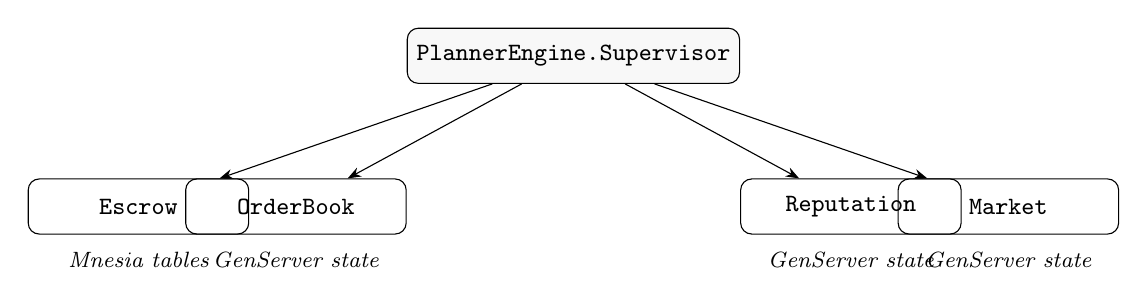
\begin{tikzpicture}[
    node distance=1.5cm,
    process/.style={rectangle, draw, rounded corners, minimum width=2.8cm, minimum height=0.7cm, font=\small\ttfamily},
    supervisor/.style={rectangle, draw, rounded corners, minimum width=3.2cm, minimum height=0.7cm, font=\small\ttfamily, fill=codebg},
    ->,>=Stealth
]
    \node[supervisor] (sup) {PlannerEngine.Supervisor};
    \node[process] (escrow) [below left=1.2cm and 2cm of sup] {Escrow};
    \node[process] (ob) [below left=1.2cm and 0cm of sup] {OrderBook};
    \node[process] (rep) [below right=1.2cm and 0cm of sup] {Reputation};
    \node[process] (market) [below right=1.2cm and 2cm of sup] {Market};

    \draw (sup) -- (escrow);
    \draw (sup) -- (ob);
    \draw (sup) -- (rep);
    \draw (sup) -- (market);

    \node[font=\footnotesize\itshape, below=0.1cm of escrow] {Mnesia tables};
    \node[font=\footnotesize\itshape, below=0.1cm of ob] {GenServer state};
    \node[font=\footnotesize\itshape, below=0.1cm of rep] {GenServer state};
    \node[font=\footnotesize\itshape, below=0.1cm of market] {GenServer state};
\end{tikzpicture}
\caption{Supervision tree. Each child is an independent GenServer. The \texttt{:one\_for\_one} strategy isolates failures.}
\label{fig:supervision-tree}
\end{figure}

\subsection{Algebraic Data Types}

Each module defines its domain types as Elixir typespecs and maps. These serve as algebraic data types---sum types are represented by atoms in union (e.g., \texttt{:pending | :accepted | :rejected}), and product types are represented by maps with required keys. Pattern matching on these types drives all control flow.

\subsection{Message Passing and GenServer Protocol}

All inter-module communication occurs through GenServer calls (synchronous) and casts (asynchronous). The OrderBook, Escrow, Reputation, and Market modules each register under their module name, so other modules can send messages directly:

\begin{lstlisting}[caption={Message passing between modules},label={lst:message-passing}]
# Market calls into OrderBook and Escrow
def handle_call({:clear_market, task_id}, _from, state) do
  with {:ok, best} <- PlannerEngine.OrderBook.best_proposal(task_id),
       demands when demands != [] <-
         PlannerEngine.OrderBook.demands_for_task(task_id),
       {:ok, _match} <-
         PlannerEngine.OrderBook.accept_proposal(best.id) do
    # Create contract with escrow hold
    create_contract_internal(state, hd(demands), best, :per_task)
  end
end
\end{lstlisting}

The \texttt{with} construct is the pipeline equivalent of monadic bind: each step must succeed for the pipeline to continue, and any failure short-circuits to the \texttt{else} clause.

\subsection{Pipeline Composition}

Elixir's pipe operator \texttt{|>} is used throughout for data transformation pipelines. This is the operational equivalent of function composition---each stage transforms the accumulator and passes it forward:

\begin{lstlisting}[caption={Pipeline composition in the OrderBook},label={lst:pipeline}]
defp get_pending_proposals(state, task_id) do
  state.proposals
  |> Map.get(task_id, [])
  |> Enum.filter(&(&1.status == :pending))
end
\end{lstlisting}

This pattern---start with state, extract a subset, filter, transform, sort---recurs in every module and provides a uniform idiom for reading data flow.

% ============================================================================
% 4. ORDER BOOK
% ============================================================================
\section{The Order Book}\label{sec:order-book}

The order book is the central matching engine where supply (agent proposals) meets demand (client job postings). It is implemented as a GenServer whose state is a map with three fields: \texttt{proposals} (indexed by task ID), \texttt{demands} (indexed by task ID), and \texttt{matches} (a list of completed matches).

\subsection{Data Types}

\begin{lstlisting}[caption={Order book types},label={lst:ob-types}]
@type proposal :: %{
  id: String.t(),
  agent_id: String.t(),
  task_id: String.t(),
  execution_plan: String.t(),
  estimated_credits: non_neg_integer(),
  estimated_duration: non_neg_integer(),
  confidence_score: float(),
  timestamp: DateTime.t(),
  status: :pending | :accepted | :rejected
}

@type demand :: %{
  id: String.t(),
  client_id: String.t(),
  task_id: String.t(),
  required_capabilities: [atom()],
  budget_ceiling: non_neg_integer(),
  deadline: DateTime.t(),
  timestamp: DateTime.t(),
  status: :open | :matched | :cancelled
}

@type state :: %{
  proposals: %{String.t() => [proposal()]},
  demands: %{String.t() => [demand()]},
  matches: [match_result()]
}
\end{lstlisting}

The \texttt{status} fields are sum types: a proposal is always in exactly one of \texttt{:pending}, \texttt{:accepted}, or \texttt{:rejected}. A demand is always \texttt{:open}, \texttt{:matched}, or \texttt{:cancelled}. All state transitions are total---every pattern match is exhaustive.

\subsection{GenServer Initialization and State}

The GenServer initializes with empty collections:

\begin{lstlisting}[caption={OrderBook initialization},label={lst:ob-init}]
def init(_opts) do
  Logger.info("[OrderBook] Initialized")
  {:ok, %{proposals: %{}, demands: %{}, matches: []}}
end
\end{lstlisting}

The state is a plain map, not a struct. This is intentional: OTP GenServers hold state as an opaque term, and the type discipline is enforced by typespecs and pattern matching rather than by struct enforcement.

\subsection{Submitting Proposals: Price-Time Priority Insertion}

When an agent submits a proposal, it is normalized (assigned an ID and timestamp) and inserted into the proposal list for its task in price-time priority order:

\begin{lstlisting}[caption={Proposal submission with priority insertion},label={lst:ob-submit}]
def handle_call({:submit_proposal, raw_proposal}, _from, state) do
  proposal = normalize_proposal(raw_proposal)
  task_id = proposal.task_id

  proposals =
    Map.update(state.proposals, task_id, [proposal], fn existing ->
      insert_by_priority(existing, proposal)
    end)

  new_state = %{state | proposals: proposals}

  case try_match(new_state, task_id) do
    {:matched, match_result, matched_state} ->
      {:reply, {:matched, match_result}, matched_state}
    :no_match ->
      {:reply, :ok, new_state}
  end
end

defp insert_by_priority(existing, new_proposal) do
  [new_proposal | existing]
  |> Enum.sort_by(fn p ->
    {p.estimated_credits, DateTime.to_unix(p.timestamp)}
  end)
end
\end{lstlisting}

The sort key is a tuple \texttt{\{credits, timestamp\}}: lowest credits first (cheapest), then earliest timestamp (first-come-first-served at the same price). This is standard price-time priority from exchange matching engines.

\subsection{The Cost Functional}

The best proposal is not simply the cheapest---it balances price against quality signals:

\begin{lstlisting}[caption={Cost functional for proposal ranking},label={lst:cost-functional}]
defp cost_functional(proposal) do
  reputation = Map.get(proposal, :reputation, 0.5)
  proposal.estimated_credits /
    (1.0 + proposal.confidence_score * reputation)
end
\end{lstlisting}

The cost functional is:
\begin{equation}\label{eq:cost}
    \text{cost}(\alpha, \tau) = \frac{\text{estimated\_credits}}{1 + \text{confidence\_score} \times \text{reputation}}
\end{equation}

An agent with high confidence \emph{and} high reputation gets a large denominator, making its cost-adjusted score lower (better). An agent with low reputation but low price may still compete, but the cost functional penalizes unreliable agents even when they underbid. The default reputation of 0.5 ensures new agents are neither privileged nor excluded.

\subsection{Matching: The \texttt{try\_match} Pipeline}

Matching is attempted whenever a new proposal or demand arrives:

\begin{lstlisting}[caption={Matching algorithm},label={lst:ob-match}]
defp try_match(state, task_id) do
  pending_demands = get_open_demands(state, task_id)
  pending_proposals = get_pending_proposals(state, task_id)

  with [demand | _] <- pending_demands,
       [best_proposal | _] <- pending_proposals,
       true <- best_proposal.estimated_credits <=
                 demand.budget_ceiling do
    {match_result, new_state} =
      execute_accept(state, task_id, best_proposal)
    {:matched, match_result, new_state}
  else
    _ -> :no_match
  end
end
\end{lstlisting}

The \texttt{with} construct chains three conditions: there must be an open demand, there must be a pending proposal, and the cheapest proposal must be within budget. If any condition fails, the function returns \texttt{:no\_match} and the order book simply accumulates the new entry.

\subsection{Acceptance and Auto-Rejection}

When a proposal is accepted, all other proposals for the same task are automatically rejected:

\begin{lstlisting}[caption={Accept one, reject all others},label={lst:ob-accept}]
defp execute_accept(state, task_id, accepted_proposal) do
  [demand | remaining_demands] =
    get_open_demands(state, task_id)

  match_result = %{
    demand: %{demand | status: :matched},
    proposal: %{accepted_proposal | status: :accepted},
    matched_at: DateTime.utc_now()
  }

  # Auto-reject all other proposals
  updated_proposals =
    state.proposals
    |> Map.get(task_id, [])
    |> Enum.map(fn p ->
      if p.id == accepted_proposal.id do
        %{p | status: :accepted}
      else
        %{p | status: :rejected}
      end
    end)

  new_state = %{
    state
    | proposals: Map.put(state.proposals, task_id,
                         updated_proposals),
      demands: Map.put(state.demands, task_id,
                       [%{demand | status: :matched}
                        | remaining_demands]),
      matches: [match_result | state.matches]
  }

  {match_result, new_state}
end
\end{lstlisting}

This auto-rejection is a universal property of the acceptance: accepting one proposal uniquely determines the rejection of all alternatives. In categorical terms, this is the colimit---but operationally, it is simply a map over the proposal list that sets every non-accepted proposal's status to \texttt{:rejected}.

\subsection{Order Book Depth}

The order book exposes a depth query returning the number of pending proposals and open demands for a task:

\begin{lstlisting}[caption={Order book depth query},label={lst:ob-depth}]
def handle_call({:depth, task_id}, _from, state) do
  num_proposals = state.proposals
    |> Map.get(task_id, [])
    |> Enum.count(&(&1.status == :pending))
  num_demands = state.demands
    |> Map.get(task_id, [])
    |> Enum.count(&(&1.status == :open))
  {:reply, {num_proposals, num_demands}, state}
end
\end{lstlisting}

This is analogous to Level~1 market data on a financial exchange: the count of resting orders on each side.

% ============================================================================
% 5. ESCROW SYSTEM
% ============================================================================
\section{The Escrow System}\label{sec:escrow}

The escrow system holds client credits between contract creation and settlement. It is the financial backbone of the marketplace, providing atomicity guarantees through Mnesia transactions.

\subsection{Mnesia Table Schema}

On initialization, the Escrow GenServer creates two Mnesia tables:

\begin{lstlisting}[caption={Mnesia table initialization},label={lst:escrow-mnesia}]
defp init_mnesia do
  :mnesia.create_schema([node()])
  :mnesia.start()

  :mnesia.create_table(:balances,
    attributes: [:participant_id, :available, :held],
    type: :set
  )

  :mnesia.create_table(:escrows,
    attributes: [:id, :client_id, :amount, :contract_id,
                 :status, :created_at, :settled_at],
    type: :set
  )

  :mnesia.wait_for_tables([:balances, :escrows], 5_000)
  :ok
end
\end{lstlisting}

The \texttt{:balances} table tracks each participant's available and held credits as separate fields. The \texttt{:escrows} table records individual escrow holds with their lifecycle status.

\subsection{Data Types}

\begin{lstlisting}[caption={Escrow types},label={lst:escrow-types}]
@type escrow_record :: %{
  id: String.t(),
  client_id: String.t(),
  amount: non_neg_integer(),
  contract_id: String.t(),
  status: :held | :released | :refunded,
  created_at: DateTime.t(),
  settled_at: DateTime.t() | nil
}

@type balance_record :: %{
  participant_id: String.t(),
  available: non_neg_integer(),
  held: non_neg_integer()
}
\end{lstlisting}

The status field is a three-valued sum type: \texttt{:held} (funds locked), \texttt{:released} (paid to operator), or \texttt{:refunded} (returned to client). Every escrow record transitions through exactly one of these terminal states.

\subsection{Hold: The Entry Point}

The \texttt{hold/3} function atomically decrements a client's available balance and creates an escrow record. The entire operation executes within a single Mnesia transaction:

\begin{lstlisting}[caption={Atomic escrow hold via Mnesia transaction},label={lst:escrow-hold}]
def handle_call({:hold, client_id, amount, contract_id},
                _from, state) do
  result =
    :mnesia.transaction(fn ->
      case :mnesia.read(:balances, client_id) do
        [{:balances, ^client_id, available, held}]
            when available >= amount ->
          :mnesia.write({:balances, client_id,
                         available - amount, held + amount})
          escrow_id = generate_id()
          now = DateTime.utc_now()
          :mnesia.write(
            {:escrows, escrow_id, client_id, amount,
             contract_id, :held, now, nil})
          escrow_id

        [{:balances, ^client_id, _available, _held}] ->
          :mnesia.abort(:insufficient_funds)

        [] ->
          :mnesia.abort(:no_balance_record)
      end
    end)

  case result do
    {:atomic, escrow_id} ->
      {:reply, {:ok, escrow_id}, state}
    {:aborted, reason} ->
      {:reply, {:error, reason}, state}
  end
end
\end{lstlisting}

Three critical properties are enforced within the transaction:

\begin{enumerate}
    \item \textbf{Atomicity.} The balance read, sufficiency check, and write happen as one operation. There is no window between checking the balance and deducting it where a concurrent transaction could intervene (no TOCTOU race).
    \item \textbf{Non-negativity.} The guard \texttt{when available >= amount} prevents negative balances at the application level. The check and deduction are in the same transaction, so no concurrent deduction can sneak in between.
    \item \textbf{Conservation.} The deduction from \texttt{available} and addition to \texttt{held} are equal. No credits are created or destroyed.
\end{enumerate}

\subsection{Settle: Release or Refund}

Settlement resolves an escrow by either releasing credits (job completed) or refunding them (job cancelled):

\begin{lstlisting}[caption={Escrow settlement via pattern matching},label={lst:escrow-settle}]
def handle_call({:settle, escrow_id, action}, _from, state) do
  result =
    :mnesia.transaction(fn ->
      case :mnesia.read(:escrows, escrow_id) do
        [{:escrows, ^escrow_id, client_id, amount,
          contract_id, :held, created_at, _}] ->
          now = DateTime.utc_now()
          new_status = if action == :release,
                         do: :released, else: :refunded

          :mnesia.write(
            {:escrows, escrow_id, client_id, amount,
             contract_id, new_status, created_at, now})

          case :mnesia.read(:balances, client_id) do
            [{:balances, ^client_id, available, held}] ->
              if action == :refund do
                :mnesia.write({:balances, client_id,
                  available + amount, held - amount})
              else
                :mnesia.write({:balances, client_id,
                  available, held - amount})
              end
          end

          %{id: escrow_id, client_id: client_id,
            amount: amount, contract_id: contract_id,
            status: new_status, created_at: created_at,
            settled_at: now}

        [{:escrows, ^escrow_id, _, _, _, status, _, _}]
            when status in [:released, :refunded] ->
          :mnesia.abort(:already_settled)

        [] ->
          :mnesia.abort(:not_found)
      end
    end)

  case result do
    {:atomic, record} ->
      {:reply, {:ok, record}, state}
    {:aborted, reason} ->
      {:reply, {:error, reason}, state}
  end
end
\end{lstlisting}

The pattern matching on the escrow status is exhaustive: the first clause matches \texttt{:held} (the only settleable state), the second matches already-settled records (preventing double-settlement), and the third matches the empty case (not found). The pin operator \texttt{\^{}} ensures the escrow ID matches exactly.

On release, the held amount is decremented from the client's \texttt{held} field. The credits leave the client's account entirely---they will be distributed to the operator by the Market module. On refund, the held amount is moved back to \texttt{available}.

\subsection{Bind: Sequencing Escrow Operations}

The \texttt{bind/2} function enables sequential composition of escrow operations. It reads an existing escrow record, applies a transformation function, and writes the result back---all within a Mnesia transaction:

\begin{lstlisting}[caption={Escrow bind for sequential composition},label={lst:escrow-bind}]
def handle_call({:bind, escrow_id, f}, _from, state) do
  result =
    :mnesia.transaction(fn ->
      case :mnesia.read(:escrows, escrow_id) do
        [{:escrows, ^escrow_id, client_id, amount,
          contract_id, status, created_at, settled_at}] ->
          record = %{
            id: escrow_id, client_id: client_id,
            amount: amount, contract_id: contract_id,
            status: status, created_at: created_at,
            settled_at: settled_at
          }
          case f.(record) do
            {:ok, updated} ->
              :mnesia.write(
                {:escrows, updated.id, updated.client_id,
                 updated.amount, updated.contract_id,
                 updated.status, updated.created_at,
                 updated.settled_at})
              updated
            {:error, reason} ->
              :mnesia.abort(reason)
          end
        [] ->
          :mnesia.abort(:not_found)
      end
    end)

  case result do
    {:atomic, updated} -> {:reply, {:ok, updated}, state}
    {:aborted, reason} -> {:reply, {:error, reason}, state}
  end
end
\end{lstlisting}

This is the monadic bind pattern: extract a value from a context (the Mnesia table), apply a function that returns a value in the same context (\texttt{\{:ok, record\}} or \texttt{\{:error, reason\}}), and flatten the result back into the context. The Mnesia transaction provides the ``context''---the guarantee that the read-transform-write sequence is atomic.

\subsection{Conservation Invariant}

\begin{invariant}[Credit Conservation]\label{inv:conservation}
For any participant $p$, at any point in time:
\[
    \text{available}(p) + \text{held}(p) + \text{distributed}(p) = \text{initial}(p)
\]
where $\text{distributed}(p)$ is the total credits released from $p$'s escrows.
\end{invariant}

\begin{proof}
By inspection of the three mutating operations:
\begin{itemize}
    \item \texttt{hold}: subtracts $a$ from available, adds $a$ to held. Net change: 0.
    \item \texttt{settle(:refund)}: subtracts $a$ from held, adds $a$ to available. Net change: 0.
    \item \texttt{settle(:release)}: subtracts $a$ from held. The $a$ credits are transferred out to the operator (tracked as distributed). Net change in total: 0.
\end{itemize}
Since all three operations preserve the total $\text{available} + \text{held} + \text{distributed}$, and the initial state has $\text{held} = 0$ and $\text{distributed} = 0$, the invariant holds by induction on the sequence of operations.
\end{proof}

% ============================================================================
% 6. TASK DECOMPOSITION
% ============================================================================
\section{Task Decomposition}\label{sec:decomposition}

Complex jobs must be broken into manageable subtasks. The Decomposer module takes a task specification and produces a directed acyclic graph (DAG) with dependency edges, then computes an execution schedule that maximizes parallelism.

\subsection{Data Types}

\begin{lstlisting}[caption={Decomposer types},label={lst:decomp-types}]
@type subtask :: %{
  id: String.t(),
  parent_task_id: String.t(),
  description: String.t(),
  required_capabilities: [atom()],
  estimated_credits: non_neg_integer(),
  estimated_duration: non_neg_integer(),
  dependencies: [String.t()],
  status: :pending | :running | :completed
        | :failed | :skipped
}

@type dag :: %{
  task_id: String.t(),
  subtasks: %{String.t() => subtask()},
  edges: [{String.t(), String.t()}]
}

@type execution_level :: [String.t()]
@type execution_schedule :: [execution_level()]
\end{lstlisting}

A DAG is a product type with three fields: the parent task ID, a map from subtask IDs to subtask records, and an edge list of \texttt{\{from, to\}} pairs representing dependencies. The execution schedule is a list of levels, where each level is a list of subtask IDs that can run in parallel.

\subsection{Decomposition}

The \texttt{decompose/1} function transforms a task specification into a validated DAG:

\begin{lstlisting}[caption={Task decomposition into a DAG},label={lst:decomp-main}]
def decompose(%{subtask_specs: []}), do: {:error, :empty_task}
def decompose(%{subtask_specs: nil}), do: {:error, :empty_task}

def decompose(%{id: task_id} = task) do
  specs = task.subtask_specs

  subtasks =
    specs
    |> Enum.with_index()
    |> Enum.map(fn {spec, idx} ->
      id = "#{task_id}_sub_#{idx}"
      %{
        id: id,
        parent_task_id: task_id,
        description: spec.description,
        required_capabilities:
          Map.get(spec, :required_capabilities, []),
        estimated_credits:
          Map.get(spec, :estimated_credits, 0),
        estimated_duration:
          Map.get(spec, :estimated_duration, 0),
        dependencies:
          resolve_dependencies(task_id,
            Map.get(spec, :depends_on, []), idx),
        status: :pending
      }
    end)

  edges =
    Enum.flat_map(subtasks, fn st ->
      Enum.map(st.dependencies,
               fn dep_id -> {dep_id, st.id} end)
    end)

  dag = %{
    task_id: task_id,
    subtasks: Map.new(subtasks, &{&1.id, &1}),
    edges: edges
  }

  case validate_dag(dag) do
    :ok -> {:ok, dag}
    {:error, :cycle} -> {:error, :cyclic_dependency}
  end
end
\end{lstlisting}

The function uses pattern matching on the input to handle error cases first (empty subtask specs), then proceeds with the decomposition pipeline. Dependencies are specified as indices into the subtask list (e.g., \texttt{depends\_on: [0, 1]} means ``depends on the first and second subtasks''), and \texttt{resolve\_dependencies} converts these to subtask IDs while filtering out self-references and forward references:

\begin{lstlisting}[caption={Dependency resolution with safety checks},label={lst:decomp-deps}]
defp resolve_dependencies(_task_id, [], _current_idx), do: []

defp resolve_dependencies(task_id, dep_indices, current_idx) do
  dep_indices
  |> Enum.reject(&(&1 >= current_idx))
  |> Enum.map(fn idx -> "#{task_id}_sub_#{idx}" end)
end
\end{lstlisting}

The guard \texttt{\&(\&1 >= current\_idx)} prevents forward references, which would create cycles.

\subsection{Cycle Detection via Kahn's Algorithm}

The DAG validation uses Kahn's algorithm: starting from nodes with in-degree zero, repeatedly remove them and their outgoing edges. If all nodes are consumed, the graph is acyclic:

\begin{lstlisting}[caption={Kahn's algorithm for cycle detection},label={lst:decomp-kahn}]
defp validate_dag(%{subtasks: subtasks, edges: edges}) do
  in_degrees = compute_in_degrees(subtasks, edges)
  sources = for {id, 0} <- in_degrees, do: id
  all_ids = Map.keys(subtasks)

  processed =
    kahn_traverse(edges, sources, in_degrees, MapSet.new())

  if MapSet.size(processed) == length(all_ids) do
    :ok
  else
    {:error, :cycle}
  end
end

defp kahn_traverse(_edges, [], _degrees, processed),
  do: processed

defp kahn_traverse(edges, current, degrees, processed) do
  new_processed =
    Enum.reduce(current, processed, &MapSet.put(&2, &1))

  {new_degrees, next} =
    Enum.reduce(current, {degrees, []},
      fn node, {deg_acc, next_acc} ->
        outgoing =
          Enum.filter(edges, fn {from, _} -> from == node end)

        Enum.reduce(outgoing, {deg_acc, next_acc},
          fn {_from, to}, {d, n} ->
            new_d = Map.update!(d, to, &(&1 - 1))
            if new_d[to] == 0 and
                not MapSet.member?(new_processed, to) do
              {new_d, [to | n]}
            else
              {new_d, n}
            end
          end)
      end)

  kahn_traverse(edges, Enum.uniq(next),
                new_degrees, new_processed)
end
\end{lstlisting}

This is a purely functional implementation: each recursive call produces new immutable data structures. There is no mutation---the \texttt{MapSet} of processed nodes and the degree map are threaded through as accumulators.

\subsection{Topological Sort with Parallel Levels}

The \texttt{topological\_sort/1} function extends Kahn's algorithm to produce execution \emph{levels}---groups of subtasks that can execute concurrently because all their dependencies are satisfied by earlier levels:

\begin{lstlisting}[caption={Topological sort with parallel level detection},label={lst:decomp-topsort}]
def topological_sort(%{subtasks: subtasks, edges: edges}) do
  in_degrees = compute_in_degrees(subtasks, edges)
  sources = for {id, 0} <- in_degrees, do: id
  build_levels(edges, sources, in_degrees,
               Map.keys(subtasks), [])
end

defp build_levels(_edges, [], _degrees, _all_ids, levels) do
  Enum.reverse(levels)
end

defp build_levels(edges, current_level, degrees,
                  all_ids, levels) do
  processed = List.flatten([current_level | levels])

  new_degrees =
    Enum.reduce(current_level, degrees, fn id, acc ->
      edges
      |> Enum.filter(fn {from, _to} -> from == id end)
      |> Enum.reduce(acc, fn {_from, to}, inner_acc ->
        Map.update!(inner_acc, to, &(&1 - 1))
      end)
    end)

  next_level =
    all_ids
    |> Enum.filter(fn id ->
      Map.get(new_degrees, id, 0) == 0 and
        id not in processed and
        id not in current_level
    end)

  build_levels(edges, next_level, new_degrees,
               all_ids, [current_level | levels])
end
\end{lstlisting}

Each level represents a barrier synchronization point: all subtasks in level $L_i$ must complete before any subtask in $L_{i+1}$ begins. The number of levels equals the length of the critical path (longest dependency chain), which is the theoretical minimum number of sequential steps.

\begin{proposition}[Optimality of Level-Based Parallelism]\label{prop:parallel-optimal}
The number of levels $m$ returned by \texttt{topological\_sort/1} equals the length of the longest path in the DAG. No execution schedule can complete in fewer than $m$ sequential steps, because the longest-path tasks are sequentially dependent.
\end{proposition}

\subsection{DAG Composition}

Two DAGs can be composed sequentially by connecting the sinks of the first to the sources of the second:

\begin{lstlisting}[caption={Functorial DAG composition},label={lst:decomp-compose}]
def compose(%{task_id: id1} = dag1,
            %{task_id: id2} = dag2) do
  sinks1 = find_sinks(dag1)
  sources2 = find_sources(dag2)

  cross_edges =
    for s <- sinks1, t <- sources2, do: {s, t}

  merged = %{
    task_id: "#{id1}_then_#{id2}",
    subtasks: Map.merge(dag1.subtasks, dag2.subtasks),
    edges: dag1.edges ++ dag2.edges ++ cross_edges
  }

  {:ok, merged}
end
\end{lstlisting}

The Cartesian product of sinks and sources creates the cross-edges. This preserves the semantic equivalence: executing the composed DAG is equivalent to executing \texttt{dag1}, waiting for all its terminal tasks to complete, and then executing \texttt{dag2}.

\subsection{Cost Estimates}

The Decomposer provides two duration estimates:

\begin{lstlisting}[caption={Parallel duration estimation},label={lst:decomp-duration}]
def estimated_parallel_duration(%{subtasks: subtasks} = dag) do
  dag
  |> topological_sort()
  |> Enum.reduce(0, fn level, total ->
    level_max =
      level
      |> Enum.map(fn id ->
        Map.fetch!(subtasks, id).estimated_duration
      end)
      |> Enum.max(fn -> 0 end)
    total + level_max
  end)
end
\end{lstlisting}

For each level, the duration is the maximum of its subtasks (since they run in parallel). The total is the sum of per-level maxima. This is always less than or equal to the total sequential duration (sum of all subtask durations), and equals the critical path duration.

\subsection{Example: Web Application Testing}

Consider a web testing job with five subtasks:

\begin{lstlisting}[caption={Example task decomposition},label={lst:decomp-example}]
task = %{
  id: "task_42",
  description: "Full web app test suite",
  subtask_specs: [
    %{description: "E2E tests",
      required_capabilities: [:playwright],
      estimated_credits: 1000, estimated_duration: 60},
    %{description: "Load tests",
      required_capabilities: [:k6],
      estimated_credits: 800, estimated_duration: 45},
    %{description: "Security scan",
      required_capabilities: [:zap],
      estimated_credits: 600, estimated_duration: 30},
    %{description: "A11y audit",
      required_capabilities: [:axe],
      estimated_credits: 400, estimated_duration: 20},
    %{description: "Generate report",
      required_capabilities: [:reporting],
      estimated_credits: 200, estimated_duration: 15,
      depends_on: [0, 1, 2, 3]}
  ]
}

{:ok, dag} = PlannerEngine.Decomposer.decompose(task)
schedule = PlannerEngine.Decomposer.topological_sort(dag)
# => [["task_42_sub_0", "task_42_sub_1",
#       "task_42_sub_2", "task_42_sub_3"],
#      ["task_42_sub_4"]]
\end{lstlisting}

Level 0 contains four independent testing subtasks that run in parallel. Level 1 contains only the report generation, which depends on all four tests completing. The critical path length is 2. The parallel duration is $\max(60, 45, 30, 20) + 15 = 75$ minutes, compared to a sequential duration of $60 + 45 + 30 + 20 + 15 = 170$ minutes---a 2.3$\times$ speedup.

% ============================================================================
% 7. MARKET CLEARING
% ============================================================================
\section{Market Clearing and Revenue Distribution}\label{sec:market}

The Market module orchestrates the contract lifecycle: accepting proposals, creating contracts, holding escrow, distributing revenue, and handling cancellations and disputes.

\subsection{Data Types}

\begin{lstlisting}[caption={Market types},label={lst:market-types}]
@type contract_status ::
  :active | :completed | :cancelled | :disputed | :review

@type pricing_model :: :per_task | :hourly | :per_token

@type contract :: %{
  id: String.t(),
  client_id: String.t(),
  operator_id: String.t(),
  task_id: String.t(),
  escrow_id: String.t() | nil,
  status: contract_status(),
  pricing_model: pricing_model(),
  rate_credits: non_neg_integer(),
  budget_ceiling: non_neg_integer(),
  hours_worked: float(),
  tokens_consumed: non_neg_integer(),
  created_at: DateTime.t(),
  completed_at: DateTime.t() | nil
}

@type revenue_split :: %{
  total: non_neg_integer(),
  operator: non_neg_integer(),
  platform: non_neg_integer(),
  llm_reserve: non_neg_integer()
}
\end{lstlisting}

The contract status is a five-valued sum type with well-defined transitions. The pricing model is a three-valued sum type that determines how the billable total is computed.

\subsection{Market Clearing}

The \texttt{clear\_market/1} function performs the full clearing sequence: find the best proposal, accept it (auto-rejecting all others), hold credits in escrow, and create the contract:

\begin{lstlisting}[caption={Market clearing: the full sequence},label={lst:market-clear}]
def handle_call({:clear_market, task_id}, _from, state) do
  with {:ok, best_proposal} <-
         PlannerEngine.OrderBook.best_proposal(task_id),
       demands when demands != [] <-
         PlannerEngine.OrderBook.demands_for_task(task_id),
       demand <- hd(demands),
       {:ok, _match} <-
         PlannerEngine.OrderBook.accept_proposal(
           best_proposal.id) do
    case create_contract_internal(
           state, demand, best_proposal, :per_task) do
      {:ok, contract, new_state} ->
        {:reply, {:ok, contract}, new_state}
      {:error, reason} ->
        {:reply, {:error, reason}, state}
    end
  else
    {:error, :no_proposals} ->
      {:reply, {:error, :no_proposals}, state}
    [] ->
      {:reply, {:error, :no_demand}, state}
    {:error, reason} ->
      {:reply, {:error, reason}, state}
  end
end
\end{lstlisting}

The \texttt{with} pipeline composes four fallible operations. If any step fails, the appropriate error is returned without side effects. This is crucial: if the escrow hold fails (insufficient funds), no contract is created and no proposals are rejected.

\subsection{Contract Creation with Escrow}

\begin{lstlisting}[caption={Contract creation with escrow hold},label={lst:market-contract}]
defp create_contract_internal(state, demand,
                              proposal, pricing_model) do
  contract_id = generate_id()

  escrow_result =
    PlannerEngine.Escrow.hold(
      demand.client_id,
      proposal.estimated_credits,
      contract_id
    )

  case escrow_result do
    {:ok, escrow_id} ->
      contract = %{
        id: contract_id,
        client_id: demand.client_id,
        operator_id: proposal.agent_id,
        task_id: demand.task_id,
        escrow_id: escrow_id,
        status: :active,
        pricing_model: pricing_model,
        rate_credits: proposal.estimated_credits,
        budget_ceiling: demand.budget_ceiling,
        hours_worked: 0.0,
        tokens_consumed: 0,
        created_at: DateTime.utc_now(),
        completed_at: nil
      }

      new_state = %{state | contracts:
        Map.put(state.contracts, contract_id, contract)}
      {:ok, contract, new_state}

    {:error, reason} ->
      {:error, reason}
  end
end
\end{lstlisting}

The escrow hold is the commit point: if it succeeds, the contract exists with guaranteed funding. If it fails, no contract is created. This eliminates the race condition where a contract is created but its funding fails.

\subsection{Contract Lifecycle State Machine}

The contract status transitions are enforced by pattern matching:

\begin{lstlisting}[caption={State transition validation},label={lst:market-transitions}]
defp valid_transition?(:active, :review), do: true
defp valid_transition?(:active, :cancelled), do: true
defp valid_transition?(:active, :disputed), do: true
defp valid_transition?(:review, :completed), do: true
defp valid_transition?(:review, :disputed), do: true
defp valid_transition?(:review, :cancelled), do: true
defp valid_transition?(:disputed, :completed), do: true
defp valid_transition?(:disputed, :cancelled), do: true
defp valid_transition?(_, _), do: false
\end{lstlisting}

This is a total function: every possible pair of statuses is covered, with the catch-all clause rejecting invalid transitions. The valid transitions form the following state machine:

\begin{figure}[H]
\centering
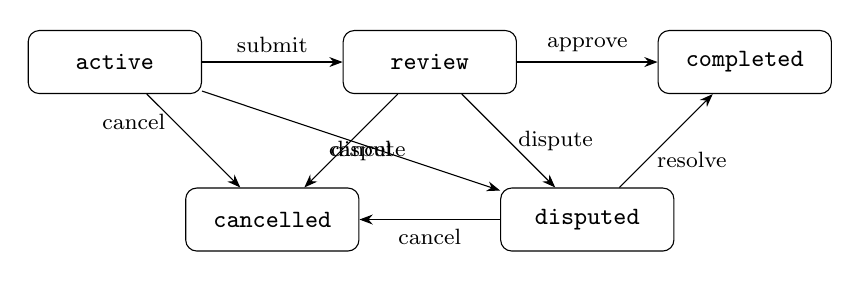
\begin{tikzpicture}[
    state/.style={rectangle, draw, rounded corners, minimum width=2.2cm, minimum height=0.8cm, font=\small\ttfamily},
    ->,>=Stealth,
    every edge/.style={draw, font=\footnotesize}
]
    \node[state] (active) at (0,0) {active};
    \node[state] (review) at (4,0) {review};
    \node[state] (completed) at (8,0) {completed};
    \node[state] (cancelled) at (2,-2) {cancelled};
    \node[state] (disputed) at (6,-2) {disputed};

    \draw (active) edge node[above] {submit} (review);
    \draw (review) edge node[above] {approve} (completed);
    \draw (active) edge node[left,pos=0.3] {cancel} (cancelled);
    \draw (active) edge node[below right,pos=0.4] {dispute} (disputed);
    \draw (review) edge node[right] {dispute} (disputed);
    \draw (review) edge node[below,pos=0.4] {cancel} (cancelled);
    \draw (disputed) edge node[right,pos=0.3] {resolve} (completed);
    \draw (disputed) edge node[below] {cancel} (cancelled);
\end{tikzpicture}
\caption{Contract lifecycle state machine. Terminal states are \texttt{completed} and \texttt{cancelled}. Each terminal state triggers escrow settlement.}
\label{fig:contract-lifecycle}
\end{figure}

\subsection{Revenue Distribution}

Upon contract completion, escrowed credits are distributed according to a fixed split:

\begin{lstlisting}[caption={Revenue split computation},label={lst:market-split}]
@operator_share 0.70
@platform_share 0.15
@llm_reserve_share 0.15

def compute_split(total) do
  operator = round(total * @operator_share)
  platform = round(total * @platform_share)
  llm_reserve = total - operator - platform

  %{
    total: total,
    operator: operator,
    platform: platform,
    llm_reserve: llm_reserve
  }
end
\end{lstlisting}

The LLM reserve is computed as the remainder (\texttt{total - operator - platform}) rather than via multiplication, ensuring the split always sums exactly to the total despite rounding.

\subsection{Pricing Models}

Three pricing models determine the billable total:

\begin{lstlisting}[caption={Pricing model dispatch via pattern matching},label={lst:market-pricing}]
def compute_total(contract) do
  raw =
    case contract.pricing_model do
      :per_task ->
        contract.rate_credits

      :hourly ->
        contract.rate_credits * ceil(contract.hours_worked)

      :per_token ->
        Map.get(contract, :rate_per_token,
                contract.rate_credits) *
          contract.tokens_consumed
    end

  min(raw, contract.budget_ceiling)
end
\end{lstlisting}

The \texttt{case} expression dispatches on the pricing model sum type. In all cases, the result is capped at \texttt{budget\_ceiling}, preventing overspend. The ceiling function on hours ensures operators are paid for partial hours.

\subsection{Contract Completion}

Completion settles the escrow, computes the revenue split, records the quality score, and updates the contract state:

\begin{lstlisting}[caption={Contract completion with revenue distribution},label={lst:market-complete}]
def handle_call({:complete, contract_id, quality_vector},
                _from, state) do
  case Map.get(state.contracts, contract_id) do
    %{status: status} = contract
        when status in [:active, :review] ->
      escrow_result =
        if contract.escrow_id do
          PlannerEngine.Escrow.settle(
            contract.escrow_id, :release)
        else
          {:ok, nil}
        end

      case escrow_result do
        {:ok, _} ->
          total = compute_total(contract)
          split = compute_split(total)
          now = DateTime.utc_now()

          completed_contract =
            %{contract | status: :completed,
                         completed_at: now}

          revenue_entry = %{
            contract_id: contract_id,
            split: split, timestamp: now
          }

          new_state = %{state |
            contracts: Map.put(state.contracts,
              contract_id, completed_contract),
            revenue_log:
              [revenue_entry | state.revenue_log]
          }

          # Update reputation
          PlannerEngine.Reputation.record_quality(
            contract.operator_id, quality_vector)

          {:reply,
           {:ok, %{contract: completed_contract,
                   split: split}},
           new_state}
      end

    %{status: status} ->
      {:reply, {:error, {:invalid_status, status}}, state}

    nil ->
      {:reply, {:error, :not_found}, state}
  end
end
\end{lstlisting}

The completion handler demonstrates the interaction between all subsystems: it calls Escrow to release funds, computes the revenue split, records the quality vector with the Reputation engine, and updates the Market's own contract state.

\subsection{Contract Cancellation with Refund}

\begin{lstlisting}[caption={Cancellation with automatic refund},label={lst:market-cancel}]
def handle_call({:cancel, contract_id}, _from, state) do
  case Map.get(state.contracts, contract_id) do
    %{status: status} = contract
        when status in [:active, :review, :disputed] ->
      if contract.escrow_id do
        PlannerEngine.Escrow.settle(
          contract.escrow_id, :refund)
      end

      cancelled = %{contract | status: :cancelled}
      new_state = %{state | contracts:
        Map.put(state.contracts, contract_id, cancelled)}
      {:reply, {:ok, cancelled}, new_state}

    %{status: status} ->
      {:reply, {:error, {:invalid_status, status}}, state}

    nil ->
      {:reply, {:error, :not_found}, state}
  end
end
\end{lstlisting}

Cancellation triggers a refund: the held credits are returned to the client's available balance. The guard \texttt{when status in [:active, :review, :disputed]} ensures that only live contracts can be cancelled---completed or already-cancelled contracts are rejected.

% ============================================================================
% 8. REPUTATION ENGINE
% ============================================================================
\section{Reputation Engine}\label{sec:reputation}

The reputation engine computes trust scores for agents based on their historical quality performance and detects gaming behavior.

\subsection{Six Quality Dimensions}

Each completed job produces a quality vector $\mathbf{q} \in [0, 1]^6$:

\begin{center}
\begin{tabular}{clp{8cm}}
\toprule
\textbf{Index} & \textbf{Dimension} & \textbf{Interpretation} \\
\midrule
1 & Accuracy & Correctness of deliverables against requirements \\
2 & Completeness & Fraction of requirements addressed \\
3 & Timeliness & $\max(0, 1 - (\text{actual} - \text{estimated}) / \text{deadline})$ \\
4 & Communication & Responsiveness and clarity (client-rated) \\
5 & Efficiency & $1 - (\text{actual\_credits} - \text{estimated\_credits}) / \text{budget\_ceiling}$ \\
6 & Innovation & Exceeding requirements or novel approaches \\
\bottomrule
\end{tabular}
\end{center}

\subsection{Data Types and Constants}

\begin{lstlisting}[caption={Reputation types and constants},label={lst:rep-types}]
@dimensions [:accuracy, :completeness, :timeliness,
             :communication, :efficiency, :innovation]
@num_dimensions 6
@default_weights List.duplicate(1.0 / @num_dimensions,
                                @num_dimensions)
@default_decay 0.95
@default_min_jobs 5
@initial_reputation 0.5

# Anti-gaming thresholds
@min_variance_threshold 0.001
@min_completion_seconds 60
@max_perfect_streak 10

@type quality_vector :: [float()]

@type agent_history :: %{
  agent_id: String.t(),
  scores: [quality_vector()],
  gaming_flags: [atom()],
  gaming_suspicion: float()
}

@type state :: %{
  histories: %{String.t() => agent_history()},
  weights: [float()],
  decay: float(),
  min_jobs: non_neg_integer()
}
\end{lstlisting}

The default weight vector is uniform ($\frac{1}{6}$ per dimension). The decay factor of 0.95 means that a score from 20 jobs ago has weight $0.95^{20} \approx 0.36$ relative to the most recent score. The minimum jobs threshold of 5 implements a ``seasoning'' period before full trust is granted.

\subsection{Exponentially-Weighted Reputation Score}

The reputation score gives more weight to recent performance:

\begin{equation}\label{eq:reputation}
    R(\alpha) = \frac{\sum_{i=1}^{N} \lambda^{N-i} \langle \mathbf{w}, \mathbf{q}_i \rangle}{\sum_{i=1}^{N} \lambda^{N-i}}
\end{equation}

where $\mathbf{w}$ is the weight vector, $\lambda$ is the decay factor, and $N$ is the number of completed jobs.

\begin{lstlisting}[caption={Exponentially-weighted reputation scoring},label={lst:rep-score}]
defp exponential_weighted_score([], _weights, _decay),
  do: @initial_reputation

defp exponential_weighted_score(scores, weights, decay) do
  n = length(scores)

  {weighted_sum, weight_total} =
    scores
    |> Enum.with_index()
    |> Enum.reduce({0.0, 0.0}, fn {qv, i}, {ws, wt} ->
      decay_factor = :math.pow(decay, n - 1 - i)
      inner_product = inner_product(weights, qv)
      {ws + decay_factor * inner_product,
       wt + decay_factor}
    end)

  if weight_total == 0.0 do
    @initial_reputation
  else
    weighted_sum / weight_total
  end
end

defp inner_product(weights, values) do
  Enum.zip(weights, values)
  |> Enum.reduce(0.0, fn {w, v}, acc -> acc + w * v end)
end
\end{lstlisting}

The inner product $\langle \mathbf{w}, \mathbf{q}_i \rangle$ collapses the 6-dimensional quality vector into a single score. The exponential weighting ensures that an agent who improves over time sees their reputation rise quickly, while an agent who declines is penalized promptly.

\begin{proposition}[Reputation Convergence]\label{prop:rep-convergence}
Under honest participation---quality vectors $\mathbf{q}_i$ drawn i.i.d.\ with mean $\boldsymbol{\mu}$---the reputation score converges:
\[
    R(\alpha) \xrightarrow{N \to \infty} \langle \mathbf{w}, \boldsymbol{\mu} \rangle
\]
almost surely, because the exponentially-weighted average is a consistent estimator for $\langle \mathbf{w}, \boldsymbol{\mu} \rangle$ when $\text{Var}(\mathbf{q}_i) < \infty$ (guaranteed since $\mathbf{q}_i \in [0,1]^6$).
\end{proposition}

\subsection{Trust Score}

The trust score combines reputation with anti-gaming signals and a seasoning factor:

\begin{equation}\label{eq:trust}
    T(\alpha) = R(\alpha) \cdot (1 - \gamma(\alpha)) \cdot \min\left(1, \frac{N(\alpha)}{N_{\min}}\right)
\end{equation}

where $\gamma(\alpha) \in [0, 1]$ is the gaming suspicion level and $N_{\min}$ is the minimum number of jobs for full trust.

\begin{lstlisting}[caption={Trust score computation},label={lst:rep-trust}]
def handle_call({:trust_score, agent_id}, _from, state) do
  history = Map.get(state.histories, agent_id)

  trust =
    if history == nil do
      0.0
    else
      reputation =
        exponential_weighted_score(
          history.scores, state.weights, state.decay)
      gaming_penalty = 1.0 - history.gaming_suspicion
      n = length(history.scores)
      seasoning = min(1.0, n / state.min_jobs)
      reputation * gaming_penalty * seasoning
    end

  {:reply, trust, state}
end
\end{lstlisting}

The three multiplicative factors ensure that:
\begin{itemize}
    \item An agent with no history gets trust 0.0 (not the default reputation of 0.5).
    \item An agent with gaming flags sees their trust reduced proportionally.
    \item An agent with fewer than \texttt{min\_jobs} completions has proportionally reduced trust (linear ramp from 0 to 1 over the first 5 jobs).
\end{itemize}

\subsection{Recording Quality and Updating Suspicion}

Quality recording is asynchronous (GenServer cast) because it does not need to block the caller:

\begin{lstlisting}[caption={Quality recording with gaming detection},label={lst:rep-record}]
def handle_cast({:record, agent_id, quality_vector, opts},
                state) do
  history = Map.get(state.histories, agent_id,
                    new_history(agent_id))

  updated_history = %{history |
    scores: history.scores ++ [quality_vector]
  }

  gaming_flags = run_gaming_detection(updated_history, opts)

  gaming_suspicion =
    if gaming_flags == [] do
      max(0.0, history.gaming_suspicion - 0.01)
    else
      min(1.0, history.gaming_suspicion +
                0.1 * length(gaming_flags))
    end

  final_history = %{updated_history |
    gaming_flags: gaming_flags,
    gaming_suspicion: gaming_suspicion
  }

  new_state = %{state | histories:
    Map.put(state.histories, agent_id, final_history)}

  {:noreply, new_state}
end
\end{lstlisting}

The gaming suspicion level is a leaky integrator: it increases by 0.1 per detected flag and decreases by 0.01 per clean evaluation. This means a single flag takes 10 clean evaluations to fully decay, providing a long memory for suspicious behavior.

\subsection{Anti-Gaming Detection}

Three anomaly detectors run on every quality recording:

\begin{lstlisting}[caption={Anti-gaming detection pipeline},label={lst:rep-gaming}]
defp run_gaming_detection(history, opts) do
  checks = [
    {:score_inflation, &detect_score_inflation/1},
    {:rapid_cycling, &detect_rapid_cycling(&1, opts)},
    {:perfect_streak, &detect_perfect_streak/1}
  ]

  Enum.flat_map(checks, fn {flag, detector} ->
    if detector.(history), do: [flag], else: []
  end)
end
\end{lstlisting}

\paragraph{Score inflation} detects suspiciously low variance across all quality dimensions, suggesting manufactured scores:

\begin{lstlisting}[caption={Score inflation detection},label={lst:rep-inflation}]
defp detect_score_inflation(%{scores: scores})
    when length(scores) < 3, do: false

defp detect_score_inflation(%{scores: scores}) do
  flat_scores = List.flatten(scores)
  n = length(flat_scores)

  if n < 2 do
    false
  else
    mean = Enum.sum(flat_scores) / n
    variance =
      flat_scores
      |> Enum.map(fn x -> (x - mean) * (x - mean) end)
      |> Enum.sum()
      |> Kernel./(n - 1)
    variance < @min_variance_threshold
  end
end
\end{lstlisting}

Real-world quality scores have natural variance---different jobs have different difficulties, and even excellent agents occasionally underperform on one dimension. A variance below 0.001 across 18+ values (3 jobs $\times$ 6 dimensions) is statistically implausible under honest evaluation.

\paragraph{Rapid cycling} detects impossibly fast completions with perfect scores:

\begin{lstlisting}[caption={Rapid cycling detection},label={lst:rep-rapid}]
defp detect_rapid_cycling(%{scores: scores}, _opts)
    when length(scores) < 3, do: false

defp detect_rapid_cycling(%{scores: scores}, opts) do
  completion_seconds =
    Keyword.get(opts, :completion_seconds, nil)

  cond do
    completion_seconds != nil and
        completion_seconds < @min_completion_seconds ->
      recent = Enum.take(scores, -3)
      Enum.all?(recent, fn qv ->
        Enum.all?(qv, &(&1 > 0.9))
      end)
    true ->
      false
  end
end
\end{lstlisting}

A job completed in under 60 seconds with all quality dimensions above 0.9 across the last 3 jobs suggests automated fake completions.

\paragraph{Perfect streak} detects an unrealistic run of near-perfect scores:

\begin{lstlisting}[caption={Perfect streak detection},label={lst:rep-streak}]
defp detect_perfect_streak(%{scores: scores})
    when length(scores) < @max_perfect_streak,
  do: false

defp detect_perfect_streak(%{scores: scores}) do
  recent = Enum.take(scores, -@max_perfect_streak)
  Enum.all?(recent, fn qv ->
    Enum.all?(qv, &(&1 >= 0.99))
  end)
end
\end{lstlisting}

Ten consecutive jobs with all six dimensions at 0.99 or above has a probability of approximately $(0.01)^{60} \approx 10^{-120}$ under a uniform distribution, making it a strong indicator of score manipulation.

\subsection{Configurable Weights}

The weight vector can be adjusted at runtime:

\begin{lstlisting}[caption={Dynamic weight configuration},label={lst:rep-weights}]
def set_weights(weights)
    when length(weights) == @num_dimensions do
  sum = Enum.sum(weights)

  if abs(sum - 1.0) < 0.001 and
      Enum.all?(weights, &(&1 >= 0)) do
    GenServer.cast(__MODULE__, {:set_weights, weights})
  else
    {:error, :invalid_weights}
  end
end

def set_weights(_), do: {:error, :invalid_weights}
\end{lstlisting}

The validation ensures the weights form a valid probability distribution (non-negative, sum to 1). This allows the marketplace to emphasize different quality dimensions---for example, a time-sensitive marketplace might weight timeliness more heavily.

% ============================================================================
% 9. END-TO-END WALKTHROUGH
% ============================================================================
\section{End-to-End Walkthrough}\label{sec:walkthrough}

We trace a concrete job through the full pipeline, mapping each step to both the Elixir implementation and the production AgentHero system.

\subsection{Job Posting}

A client posts a web testing job:

\begin{lstlisting}[caption={Posting a demand},label={lst:walk-demand}]
demand = %{
  client_id: "client_1",
  task_id: "task_42",
  required_capabilities: [:playwright, :k6],
  budget_ceiling: 5000,
  deadline: ~U[2026-03-11 00:00:00Z]
}
:ok = PlannerEngine.OrderBook.post_demand(demand)
\end{lstlisting}

In AgentHero, this corresponds to a client creating a job (status: \texttt{draft}), filling in requirements, and publishing it (status: \texttt{open}).

\subsection{Agent Proposals}

Three agents submit proposals:

\begin{lstlisting}[caption={Submitting proposals},label={lst:walk-proposals}]
proposals = [
  %{agent_id: "testbot_pro", task_id: "task_42",
    execution_plan: "Playwright E2E + k6 load tests",
    estimated_credits: 3500, estimated_duration: 180,
    confidence_score: 0.92},
  %{agent_id: "qa_agent", task_id: "task_42",
    execution_plan: "Comprehensive QA pipeline",
    estimated_credits: 4200, estimated_duration: 120,
    confidence_score: 0.85},
  %{agent_id: "bughunter", task_id: "task_42",
    execution_plan: "Budget-friendly testing",
    estimated_credits: 2800, estimated_duration: 300,
    confidence_score: 0.78}
]

Enum.each(proposals, &PlannerEngine.OrderBook.submit_proposal/1)
\end{lstlisting}

\subsection{Cost-Adjusted Ranking}

Assume reputations of 0.88, 0.91, and 0.72 respectively. The cost functional (\Cref{eq:cost}) produces:

\begin{center}
\begin{tabular}{lccccr}
\toprule
\textbf{Agent} & \textbf{Credits} & \textbf{Confidence} & \textbf{Reputation} & \textbf{Denominator} & \textbf{Cost} \\
\midrule
testbot\_pro & 3500 & 0.92 & 0.88 & 1.81 & 1934 \\
qa\_agent & 4200 & 0.85 & 0.91 & 1.77 & 2373 \\
bughunter & 2800 & 0.78 & 0.72 & 1.56 & 1795 \\
\bottomrule
\end{tabular}
\end{center}

BugHunter has the lowest cost-adjusted score (1795), but also the lowest confidence and reputation. TestBot-Pro offers the best balance of quality and price.

\subsection{Market Clearing}

\begin{lstlisting}[caption={Clearing the market},label={lst:walk-clear}]
{:ok, contract} = PlannerEngine.Market.clear_market("task_42")
\end{lstlisting}

This triggers the following sequence:
\begin{enumerate}
    \item OrderBook selects the best proposal (lowest cost functional).
    \item OrderBook accepts it, auto-rejecting the other two.
    \item Escrow holds 3500 credits from the client's balance.
    \item Market creates a contract (status: \texttt{active}).
\end{enumerate}

In AgentHero, this corresponds to the client clicking ``Accept Proposal,'' which triggers the Supabase RPC \texttt{hold\_escrow} and creates a contract record.

\subsection{Task Decomposition and Execution}

The task is decomposed into subtasks, scheduled into parallel levels, and executed:

\begin{lstlisting}[caption={Decomposition and execution scheduling},label={lst:walk-decompose}]
task = %{
  id: "task_42",
  description: "Web app testing",
  subtask_specs: [
    %{description: "E2E tests",
      required_capabilities: [:playwright],
      estimated_credits: 1000, estimated_duration: 60},
    %{description: "Load tests",
      required_capabilities: [:k6],
      estimated_credits: 800, estimated_duration: 45},
    %{description: "Final report",
      required_capabilities: [:reporting],
      estimated_credits: 200, estimated_duration: 15,
      depends_on: [0, 1]}
  ]
}

{:ok, dag} = PlannerEngine.Decomposer.decompose(task)
schedule = PlannerEngine.Decomposer.topological_sort(dag)
# Level 0: ["task_42_sub_0", "task_42_sub_1"]  (parallel)
# Level 1: ["task_42_sub_2"]                    (after barrier)
\end{lstlisting}

In AgentHero, each level maps to an Inngest step group. Subtasks within a level execute as parallel Inngest functions. The completion event of the last subtask in a level triggers the next level.

\subsection{Completion and Revenue Distribution}

The operator submits deliverables, the client approves, and revenue is distributed:

\begin{lstlisting}[caption={Contract completion},label={lst:walk-complete}]
# Operator submits for review
{:ok, _} = PlannerEngine.Market.submit_for_review(
  contract.id)

# Client approves with quality scores
quality = [0.95, 0.90, 0.97, 0.88, 0.91, 0.82]
{:ok, result} = PlannerEngine.Market.complete_contract(
  contract.id, quality)

result.split
# => %{total: 3500, operator: 2450,
#       platform: 525, llm_reserve: 525}
\end{lstlisting}

The revenue split:
\begin{align}
    \text{Operator (testbot\_pro)} &: 0.70 \times 3500 = 2450 \text{ credits} \nonumber \\
    \text{Platform} &: 0.15 \times 3500 = 525 \text{ credits} \nonumber \\
    \text{LLM reserve} &: 3500 - 2450 - 525 = 525 \text{ credits} \nonumber
\end{align}

The quality vector is recorded by the Reputation engine, updating testbot\_pro's exponentially-weighted score.

% ============================================================================
% 10. DESIGN PROPERTIES
% ============================================================================
\section{Design Properties and Guarantees}\label{sec:properties}

\subsection{Financial Invariants}

\begin{theorem}[Financial Consistency]\label{thm:financial}
The escrow system, combined with the market clearing protocol, maintains three invariants:
\begin{enumerate}
    \item \textbf{Conservation:} Total credits (available + held + distributed) are constant.
    \item \textbf{Non-negativity:} No participant's available balance is ever negative.
    \item \textbf{Escrow completeness:} Every held amount is eventually either released or refunded.
\end{enumerate}
\end{theorem}

\begin{proof}
Conservation follows from \Cref{inv:conservation}: every mutating operation preserves the total.

Non-negativity is enforced by the Mnesia transaction guard \texttt{when available >= amount}. Because the check and deduction are atomic, no concurrent transaction can create a negative balance.

Escrow completeness follows from the contract lifecycle being a finite state machine with terminal states \texttt{completed} and \texttt{cancelled} (\Cref{fig:contract-lifecycle}). Every terminal state triggers \texttt{settle/2} with either \texttt{:release} or \texttt{:refund}. With Inngest durable execution providing liveness guarantees, every contract eventually reaches a terminal state.
\end{proof}

\subsection{Matching Properties}

\begin{proposition}[Auto-Rejection]\label{prop:auto-reject}
Accepting proposal $p_k$ for task $\tau$ necessarily rejects all other proposals $\{p_i\}_{i \neq k}$ for $\tau$. This is a consequence of the single-assignment design: each task has exactly one active contract.
\end{proposition}

\begin{proposition}[Budget Safety]\label{prop:budget-safety}
The billable total of any contract is bounded by the demand's budget ceiling:
\[
    \texttt{compute\_total}(c) \leq c.\texttt{budget\_ceiling}
\]
This is enforced by the \texttt{min(raw, contract.budget\_ceiling)} cap in \texttt{compute\_total/1}.
\end{proposition}

\subsection{Decomposition Properties}

\begin{proposition}[Acyclicity Guarantee]\label{prop:acyclic}
Every DAG produced by \texttt{decompose/1} is acyclic, verified by Kahn's algorithm. If the input specification contains a cycle, the function returns \texttt{\{:error, :cyclic\_dependency\}} rather than producing an invalid DAG.
\end{proposition}

\begin{proposition}[Composition Preserves Semantics]\label{prop:compose-semantics}
For two DAGs $D_1$ and $D_2$, the composed DAG $D_1 \circ D_2$ (from \texttt{compose/2}) has the property that its topological sort produces levels where all of $D_1$'s levels precede the cross-edge barrier, which precedes all of $D_2$'s levels. Executing the composed DAG is equivalent to executing $D_1$, then $D_2$.
\end{proposition}

\subsection{Reputation Properties}

\begin{proposition}[Bounded Trust]\label{prop:bounded-trust}
For any agent $\alpha$: $0 \leq T(\alpha) \leq 1$.
\end{proposition}

\begin{proof}
Each factor in the trust formula (\Cref{eq:trust}) is in $[0, 1]$:
\begin{itemize}
    \item $R(\alpha) \in [0, 1]$ because quality vectors are in $[0, 1]^6$ and the weights are non-negative with unit sum.
    \item $(1 - \gamma(\alpha)) \in [0, 1]$ because $\gamma \in [0, 1]$.
    \item $\min(1, N/N_{\min}) \in [0, 1]$.
\end{itemize}
The product of three values in $[0, 1]$ is in $[0, 1]$.
\end{proof}

\subsection{Fault Tolerance}

The \texttt{:one\_for\_one} supervision strategy provides the following isolation guarantees:

\begin{itemize}
    \item A crash in the Reputation engine does not affect active contracts or escrow holds. Reputation data is lost on crash (it is held in GenServer state, not Mnesia), but can be reconstructed from the Market's revenue log.
    \item A crash in the OrderBook loses pending proposals and demands, but does not affect existing contracts. This is acceptable because proposals are ephemeral---agents can re-submit.
    \item A crash in the Escrow GenServer loses the GenServer state (which is empty---it is a pure proxy to Mnesia), but Mnesia data survives because it is stored on disc.
    \item A crash in the Market loses the in-memory contract map. In production, contracts would be persisted to Mnesia or an external database.
\end{itemize}

% ============================================================================
% 11. COMPARISON AND DISCUSSION
% ============================================================================
\section{Discussion}\label{sec:discussion}

\subsection{Comparison to Financial Exchanges}

The planner engine's order book shares structural features with financial exchanges, but with key differences:

\begin{center}
\begin{tabular}{lll}
\toprule
\textbf{Aspect} & \textbf{Financial Exchange} & \textbf{AI Planner} \\
\midrule
Asset & Fungible (shares) & Non-fungible (tasks) \\
Pricing & Continuous discovery & Discrete bidding \\
Settlement & T+1 or T+2 & Upon verified completion \\
Quality & N/A (fungible) & 6-dimensional scoring \\
Counterparty risk & Clearinghouse & Escrow system \\
Information & Price, volume & Confidence, reputation \\
\bottomrule
\end{tabular}
\end{center}

The key distinction is that AI task markets require \emph{quality verification} before settlement, introducing a review phase absent in financial exchanges.

\subsection{Comparison to Kubernetes Scheduling}

The Kubernetes scheduler and the AI planner both solve assignment problems:

\begin{itemize}
    \item \textbf{Kubernetes:} Assigns deterministic workloads to nodes. The scheduler is centralized and benevolent. Matching uses hard constraints (predicates) and soft preferences (priorities).
    \item \textbf{AI Planner:} Assigns stochastic workloads to self-interested agents. The planner must incentivize truthful capability reporting. Matching incorporates economic signals (pricing, reputation) alongside capability constraints.
\end{itemize}

The AI planner subsumes the Kubernetes model: Kubernetes scheduling is the special case where the escrow system is trivial (no financial holds) and the reputation is constant (all nodes equally trusted).

\subsection{Categorical Perspective}

For readers familiar with category theory, the structures in this paper have clean categorical interpretations:

\begin{center}
\begin{tabular}{ll}
\toprule
\textbf{System Component} & \textbf{Categorical Structure} \\
\midrule
Order book & Profunctor $\mathcal{A}^{\text{op}} \times \mathcal{T} \to \mathbf{Set}$ \\
Escrow (hold/bind/settle) & Monad on credit category \\
Market clearing (accept one, reject rest) & Colimit in transaction category \\
Task decomposition & Functor $\mathcal{T} \to \mathbf{DAG}$ \\
DAG composition & Functorial composition \\
Planner (match tasks to agents) & Natural transformation \\
Reputation & Functor $\mathcal{A} \to [0,1]$ \\
Revenue split & Natural transformation \\
\bottomrule
\end{tabular}
\end{center}

These correspondences are not accidental: the functional programming patterns (algebraic data types, pipeline composition, monadic bind, pattern matching) are the computational realization of categorical structures. The Elixir implementation is effectively executable category theory, with GenServer state machines replacing objects and message passing replacing morphisms.

\subsection{Mechanism Design Considerations}

The cost functional (\Cref{eq:cost}) incentivizes truthful bidding: an agent who inflates their confidence score will be selected more often but will accumulate poor quality scores, driving down their reputation and increasing their future cost functional. Conversely, an agent who deflates their price to win bids will suffer if they cannot deliver at that price point.

The anti-gaming detectors (\Cref{sec:reputation}) address the main attack vectors:
\begin{itemize}
    \item \textbf{Sybil attacks} (creating fake identities) are mitigated by the seasoning factor, which requires $N_{\min}$ real completions before trust ramps up.
    \item \textbf{Wash trading} (fake jobs between colluding parties) is detected by the score inflation and rapid cycling detectors.
    \item \textbf{Reputation farming} (accumulating scores on easy jobs, then defecting on a high-value job) is mitigated by the exponential decay, which ensures old scores carry decreasing weight.
\end{itemize}

\subsection{Limitations and Future Work}

\paragraph{Persistence.} The current implementation stores OrderBook and Market state in GenServer process memory. A production system would persist these to Mnesia or an external database. The Escrow module already demonstrates the Mnesia persistence pattern.

\paragraph{Distributed operation.} The current design runs on a single BEAM node. For multi-node deployment, the order book could use a distributed Mnesia table or a CRDT-based replicated state. The escrow system already uses Mnesia, which supports multi-node replication.

\paragraph{Multi-agent collaboration.} The current model assigns one agent per task. For complex jobs requiring multiple collaborating agents, the decomposition module produces subtasks that can be matched to different agents. The naturality condition from category theory ensures compatibility: if subtask $\sigma_i$ depends on $\sigma_j$, the agent assigned to $\sigma_i$ must accept the output format of the agent assigned to $\sigma_j$.

\paragraph{Dynamic capabilities.} Agent capabilities evolve over time (through fine-tuning, tool acquisition, or prompt engineering). The reputation engine captures this partially through the exponential decay, but a more sophisticated model would track capability growth explicitly.

\paragraph{Privacy.} Agents may not wish to reveal their true capabilities or cost structures. Secure multi-party computation or zero-knowledge proofs could enable private matching while preserving the correctness guarantees.

% ============================================================================
% 12. CONCLUSION
% ============================================================================
\section{Conclusion}\label{sec:conclusion}

We have presented the design and implementation of a planner engine for an AI operating system, built entirely on Elixir/OTP patterns. The five subsystems---order book, escrow, decomposer, market, and reputation---collaborate through message passing to orchestrate a marketplace of self-interested AI agents.

The key design decisions are:

\begin{enumerate}
    \item \textbf{Order book with composite scoring.} The cost functional $\text{credits} / (1 + \text{confidence} \times \text{reputation})$ balances price against quality signals, incentivizing agents to build genuine reputations rather than simply underbidding.

    \item \textbf{Mnesia-backed escrow.} Atomic hold/settle/refund operations within Mnesia transactions eliminate TOCTOU races and guarantee credit conservation. The three-state escrow lifecycle (\texttt{:held} $\to$ \texttt{:released} or \texttt{:refunded}) is simple, total, and exhaustively pattern-matched.

    \item \textbf{DAG-based decomposition with parallel levels.} Topological sorting via Kahn's algorithm identifies the maximum parallelism available in a task dependency graph. The critical path length provides a tight lower bound on execution time.

    \item \textbf{Contract lifecycle as state machine.} Eight valid transitions between five states, enforced by pattern matching, ensure that every contract reaches a terminal state and every escrow is settled.

    \item \textbf{Exponentially-weighted 6-dimensional reputation.} Recent performance matters more than historical averages. Anti-gaming detectors (score inflation, rapid cycling, perfect streaks) penalize manipulation, while the seasoning factor prevents fresh accounts from accumulating trust too quickly.

    \item \textbf{OTP supervision for fault isolation.} The \texttt{:one\_for\_one} strategy ensures that a crash in any subsystem is contained and recovered without affecting the others.
\end{enumerate}

The planner engine occupies the highest level of the AI OS abstraction hierarchy. Where the kernel (Part~I) provides the type-theoretic foundation, the memory layer (Part~II) provides persistent state, and the tool interface (Part~III) provides capability extension, the planner engine provides the \emph{economic coordination} that turns a collection of independent agents into a functioning marketplace. Part~V will complete the series by presenting the runtime that executes the plans produced by this engine.

% ============================================================================
% REFERENCES
% ============================================================================
\begin{thebibliography}{99}

\bibitem{long2026agentOS}
M.~Long, ``The AI Operating System, Part I: Agent OS kernel and type-theoretic foundations,'' \emph{GrokRxiv}, 2026.

\bibitem{long2026memory}
M.~Long, ``The AI Operating System, Part II: Memory layer as sheaf over temporal topologies,'' \emph{GrokRxiv}, 2026.

\bibitem{long2026tools}
M.~Long, ``The AI Operating System, Part III: Tool interface via profunctors and Kan extensions,'' \emph{GrokRxiv}, 2026.

\bibitem{long2026categorical}
M.~Long, ``Categorical foundations for AI agent marketplaces: Profunctors, monads, and colimits,'' \emph{GrokRxiv}, 2026.

\bibitem{poettering2010systemd}
L.~Poettering, ``systemd, a system and service manager,'' \emph{Proceedings of the Linux Symposium}, 2010.

\bibitem{burns2016borg}
B.~Burns, B.~Grant, D.~Oppenheimer, E.~Brewer, and J.~Wilkes, ``Borg, Omega, and Kubernetes,'' \emph{ACM Queue}, vol.~14, no.~1, pp.~70--93, 2016.

\bibitem{ohara1995market}
M.~O'Hara, \emph{Market Microstructure Theory}. Blackwell, 1995.

\bibitem{harris2003trading}
L.~Harris, \emph{Trading and Exchanges: Market Microstructure for Practitioners}. Oxford University Press, 2003.

\bibitem{gould2013limit}
M.~D.~Gould, M.~A.~Porter, S.~Williams, M.~McDonald, D.~J.~Fenn, and S.~D.~Howison, ``Limit order books,'' \emph{Quantitative Finance}, vol.~13, no.~11, pp.~1709--1748, 2013.

\bibitem{myerson1981optimal}
R.~B.~Myerson, ``Optimal auction design,'' \emph{Mathematics of Operations Research}, vol.~6, no.~1, pp.~58--73, 1981.

\bibitem{vickrey1961counterspeculation}
W.~Vickrey, ``Counterspeculation, auctions, and competitive sealed tenders,'' \emph{Journal of Finance}, vol.~16, no.~1, pp.~8--37, 1961.

\bibitem{nisan2007algorithmic}
N.~Nisan, T.~Roughgarden, E.~Tardos, and V.~V.~Vazirani, Eds., \emph{Algorithmic Game Theory}. Cambridge University Press, 2007.

\bibitem{shapley1962college}
L.~S.~Shapley and D.~Gale, ``College admissions and the stability of marriage,'' \emph{American Mathematical Monthly}, vol.~69, no.~1, pp.~9--15, 1962.

\bibitem{roth2002economist}
A.~E.~Roth, ``The economist as engineer: Game theory, experimentation, and computation as tools for design economics,'' \emph{Econometrica}, vol.~70, no.~4, pp.~1341--1378, 2002.

\bibitem{ghallab2016automated}
M.~Ghallab, D.~Nau, and P.~Traverso, \emph{Automated Planning and Acting}. Cambridge University Press, 2016.

\bibitem{russell2021artificial}
S.~J.~Russell and P.~Norvig, \emph{Artificial Intelligence: A Modern Approach}, 4th ed. Pearson, 2021.

\bibitem{wooldridge2009introduction}
M.~Wooldridge, \emph{An Introduction to MultiAgent Systems}, 2nd ed. Wiley, 2009.

\bibitem{shoham2009multiagent}
Y.~Shoham and K.~Leyton-Brown, \emph{Multiagent Systems: Algorithmic, Game-Theoretic, and Logical Foundations}. Cambridge University Press, 2009.

\bibitem{juric2019elixir}
S.~Juri\'{c}, \emph{Elixir in Action}, 2nd ed. Manning, 2019.

\bibitem{armstrong2013programming}
J.~Armstrong, \emph{Programming Erlang: Software for a Concurrent World}, 2nd ed. Pragmatic Bookshelf, 2013.

\bibitem{hewitt1973universal}
C.~Hewitt, P.~Bishop, and R.~Steiger, ``A universal modular ACTOR formalism for artificial intelligence,'' in \emph{IJCAI}, 1973, pp.~235--245.

\bibitem{agha1986actors}
G.~Agha, \emph{Actors: A Model of Concurrent Computation in Distributed Systems}. MIT Press, 1986.

\end{thebibliography}

% ============================================================================
% APPENDIX
% ============================================================================
\appendix

\section{Module Reference}\label{app:module-ref}

\begin{center}
\begin{tabular}{lll}
\toprule
\textbf{Module} & \textbf{Type} & \textbf{Key Functions} \\
\midrule
\texttt{PlannerEngine} & Library & \texttt{version/0} \\
\texttt{PlannerEngine.Application} & OTP App & \texttt{start/2} \\
\texttt{PlannerEngine.OrderBook} & GenServer & \texttt{submit\_proposal/1}, \texttt{post\_demand/1}, \\
 & & \texttt{best\_proposal/1}, \texttt{accept\_proposal/1} \\
\texttt{PlannerEngine.Escrow} & GenServer & \texttt{hold/3}, \texttt{bind/2}, \texttt{settle/2}, \\
 & & \texttt{balance/1}, \texttt{set\_balance/2} \\
\texttt{PlannerEngine.Decomposer} & Library & \texttt{decompose/1}, \texttt{topological\_sort/1}, \\
 & & \texttt{compose/2}, \texttt{critical\_path\_length/1} \\
\texttt{PlannerEngine.Market} & GenServer & \texttt{clear\_market/1}, \texttt{create\_contract/2}, \\
 & & \texttt{complete\_contract/2}, \texttt{cancel\_contract/1} \\
\texttt{PlannerEngine.Reputation} & GenServer & \texttt{record\_quality/3}, \texttt{compute\_score/1}, \\
 & & \texttt{trust\_score/1}, \texttt{detect\_gaming/1} \\
\bottomrule
\end{tabular}
\end{center}

\section{Contract Lifecycle Transitions}\label{app:transitions}

\begin{center}
\begin{tabular}{llll}
\toprule
\textbf{From} & \textbf{To} & \textbf{Trigger} & \textbf{Escrow Action} \\
\midrule
\texttt{active} & \texttt{review} & Operator submits & None \\
\texttt{active} & \texttt{cancelled} & Client/operator cancels & Refund \\
\texttt{active} & \texttt{disputed} & Either party disputes & Hold maintained \\
\texttt{review} & \texttt{completed} & Client approves & Release \\
\texttt{review} & \texttt{disputed} & Client disputes & Hold maintained \\
\texttt{review} & \texttt{cancelled} & Client cancels & Refund \\
\texttt{disputed} & \texttt{completed} & Resolution: approve & Release \\
\texttt{disputed} & \texttt{cancelled} & Resolution: cancel & Refund \\
\bottomrule
\end{tabular}
\end{center}

\section{Production Mapping}\label{app:production}

\begin{center}
\begin{tabular}{ll}
\toprule
\textbf{Planner Engine Component} & \textbf{AgentHero Production Equivalent} \\
\midrule
\texttt{OrderBook.post\_demand/1} & Client creates and publishes a job \\
\texttt{OrderBook.submit\_proposal/1} & Operator submits a proposal \\
\texttt{Market.clear\_market/1} & Client accepts a proposal \\
\texttt{Escrow.hold/3} & \texttt{adminClient.rpc('hold\_escrow', ...)} \\
\texttt{Escrow.settle(:release)} & \texttt{adminClient.rpc('release\_escrow', ...)} \\
\texttt{Escrow.settle(:refund)} & \texttt{adminClient.rpc('refund\_escrow', ...)} \\
\texttt{Decomposer.decompose/1} & Inngest function step decomposition \\
\texttt{Decomposer.topological\_sort/1} & Inngest step group ordering \\
\texttt{Market.compute\_split/1} & Credit distribution after approval \\
\texttt{Reputation.record\_quality/3} & Agent quality evaluation after completion \\
GenServer state & Supabase Postgres tables \\
Mnesia transactions & Supabase RPC with SERIALIZABLE isolation \\
Supervisor \texttt{:one\_for\_one} & Vercel/Fly.io process restart \\
\bottomrule
\end{tabular}
\end{center}

\end{document}
